 \documentclass{beamer}

\usepackage[utf8]{inputenc}
\usepackage[russian]{babel}
\usepackage{cmap}

\mode<presentation> {
\usetheme{Madrid}
\setbeamertemplate{caption}[numbered]
}

\usepackage{graphicx} % Allows including images
\usepackage{booktabs} % Allows the use of \toprule, \midrule and \bottomrule in tables

\title[Теория распознавания образов]{Мультибиометрическое распознавание \\ с использованием изображений лица и уха}

\author{Дедков С.В. 63501/3}
\institute[СПб ПУ]
{
Санкт-Петербургский государственный политехнический университет \\
\medskip
\textit{https://github.com/dsvgit/recognition}
}
\date{\today}

\begin{document}

\begin{frame}
\titlepage
\end{frame}

\begin{frame}
\frametitle{Содержание}
\tableofcontents
\end{frame}

%------------------------------------------------
\section{Основные понятия}
%------------------------------------------------

\begin{frame}
\frametitle{Основные понятия}

\begin{itemize}

\item[-] Место: часть тела, которую необходимо распознать (например, ухо)
\item[-] Сенсор: механизм для получения биометрической информации (например, камера)
\item[-] Алгоритм: процедура сопоставления между биометрическими сигнатурами
\item[-] Режим: комбинация места, сенсора и алгоритма
\item[-] Мульти-экземпляр: использование нескольких наборов данных полученных используя какое-либо место, сенсор и режим
\item[-] Мульти-сенсор: использование нескольких сенсоров(и возможно, алгоритмов) для захвата данных какого-либо места
\item[-] Мульти-алгоритм: использование нескольких алгоритмов сопоставления на одних и тех же данных

\end{itemize}

\end{frame}

%------------------------------------------------
\section{Слияние в мультибиометрии}
%------------------------------------------------

\begin{frame}
\frametitle{Слияние в мультибиометрии}

Мультибиометрия подразумевает слияние данных на одном из уровне распознавания. 
Способ комбинации будет влиять на качество распознавания системы.

\begin{figure}[h!]
\centering
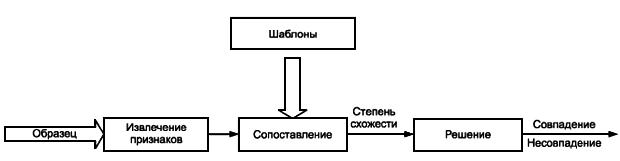
\includegraphics[scale=0.50]{res/bio_process}
\caption{Элементарный (универсальный) биометрический процесс}
\end{figure}


\end{frame}

%------------------------------------------------
\section{Варианты слияния}
%------------------------------------------------

\begin{frame}
\frametitle{Варианты слияния}

\begin{itemize}
\item объединение на уровне принятия решения
\item уровень степеней схожести
\item уровень признаков
\item уровень образцов
\end{itemize}

\end{frame}

\begin{frame}
\frametitle{Уровень принятия решения}

\begin{figure}[h!]
\centering
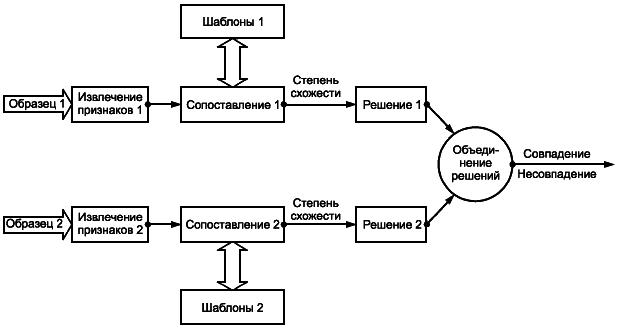
\includegraphics[scale=0.50]{res/bio_a}
\caption{объединение на уровне принятия решения}
\end{figure}

\end{frame}

\begin{frame}
\frametitle{Уровень степеней схожести}

\begin{figure}[h!]
\centering
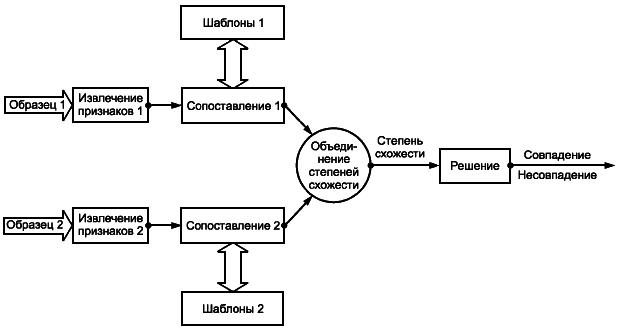
\includegraphics[scale=0.50]{res/bio_b}
\caption{объединение на уровне степеней схожести}
\end{figure}

\end{frame}

\begin{frame}
\frametitle{Уровень признаков}

\begin{figure}[h!]
\centering
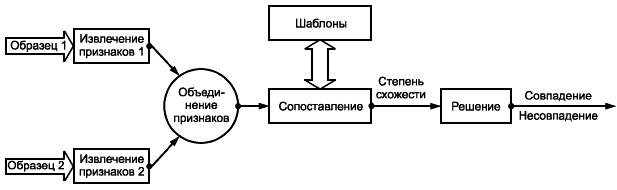
\includegraphics[scale=0.50]{res/bio_c}
\caption{объединение на уровне признаков}
\end{figure}

\end{frame}

\begin{frame}
\frametitle{Уровень образцов}

\begin{figure}[h!]
\centering
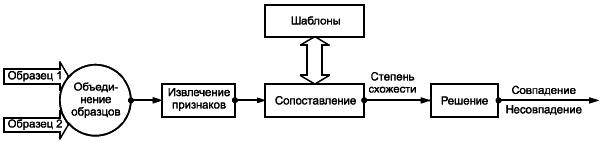
\includegraphics[scale=0.50]{res/bio_d}
\caption{объединение на уровне образцов}
\end{figure}

\end{frame}

%------------------------------------------------
\section{Метод Главных Компонент - Principal Component Analysis (PCA)}
%------------------------------------------------

\begin{frame}
\frametitle{Метод Главных Компонент - Principal Component Analysis (PCA)}

В задаче распознавания лиц PCA применяют для представления изображения лица вектором малой размерности (главных компонент), который сравнивается затем с эталонными векторами, заложенными в базу данных.

\begin{itemize}
\item обучающий набор лиц преобразуется в одну общую матрицу данных, где каждая строка представляет собой один экземпляр изображения лица, разложенного в строку
\item нормировка данных и приведение строк к 0-му среднему и 1-й дисперсии, вычисляется матрица ковариации.
\item Для полученной матрицы ковариации решается задача определения собственных значений и соответствующих им собственных векторов (собственные лица)
\item Далее производится сортировка собственных векторов в порядке убывания собственных значений и оставляют только первые k векторов
\end{itemize}

\end{frame}


%------------------------------------------------
\section{Алгоритм РСА}
%------------------------------------------------

\begin{frame}
\frametitle{Алгоритм РСА}

\begin{figure}[h!]
\centering
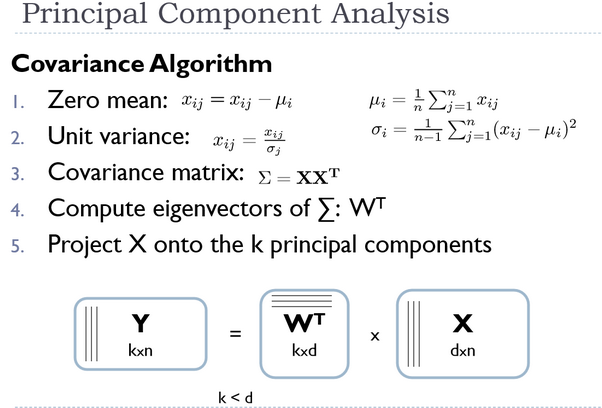
\includegraphics[scale=0.50]{res/pca_rules}
\caption{Алгоритм РСА}
\end{figure}

\end{frame}

%------------------------------------------------
\section{Принцип выбора базиса из первых лучших собственных векторов}
%------------------------------------------------

\begin{frame}
\frametitle{Принцип выбора базиса из первых лучших собственных векторов}

\begin{figure}[h!]
\centering
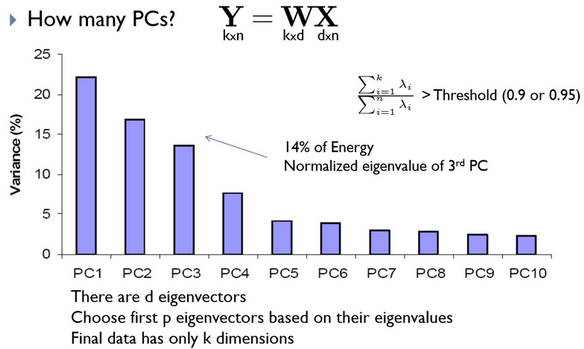
\includegraphics[scale=0.50]{res/pick_bases}
\caption{Принцип выбора базиса из первых лучших собственных векторов}
\end{figure}

\end{frame}

%------------------------------------------------
\section{2D распознавание уха}
%------------------------------------------------

\begin{frame}
\frametitle{2D распознавание уха}

Основные методы для распознавания ушей - PCA, преобразование силового поля(force field transformation), диаграммы Вороного, нейронные сети и генетические алгоритмы.

\begin{figure}[h!]
\centering
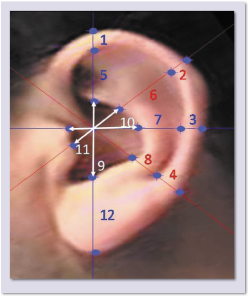
\includegraphics[scale=0.50]{res/twelve_parts}
\caption{В системе идентификации Янарелли используются 12 геометрических измерений, центральным элементом которых является ножка завитка}
\end{figure}

\end{frame}

%------------------------------------------------
\section{3D распознавание лица}
%------------------------------------------------

\begin{frame}
\frametitle{3D распознавание лица}

Сенсорные технологии:
\begin{itemize}
\item Стерео.
\item Структурированный свет.
\item Лазерное сканирование. 
\end{itemize}

Способы получения трехмерной информации о лице:
\begin{itemize}
\item Восстановление формы по теням (shape from shading, SFS)
\item Восстановление формы по стереопаре (shape from stereo)
\item Восстановление формы по движению (shape from motion, SFM)
\end{itemize}

Подходы 3D распознавания:
\begin{itemize}
\item Анализ формы 3D поверхности. 
\item Статистические методы.
\item Использование параметрической модели лица.
\end{itemize}

\end{frame}

%------------------------------------------------
\section{3D распознавание уха}
%------------------------------------------------

\begin{frame}
\frametitle{3D распознавание уха}

Для 3D распознавания уха применяют ICP алгоритм. Итеративный алгоритм ближайших точек (англ. Iterative Closest Point — ICP) — алгоритм, использующийся для сведения к минимуму разницы между двумя облаками точек.

3 этапа распознавания:
\begin{itemize}
\item автоматическое определение спирали уха
\item первый шаг ICP алгоритма для выравнивания спирали модели уха со спиралью тестового уха и получение изометрии
\item второй шаг ICP алгоритма для получения результата трансформации
\end{itemize}

\end{frame}

\begin{frame}
\frametitle{Подход к 3D распознаванию уха}

\begin{figure}[h!]
\centering
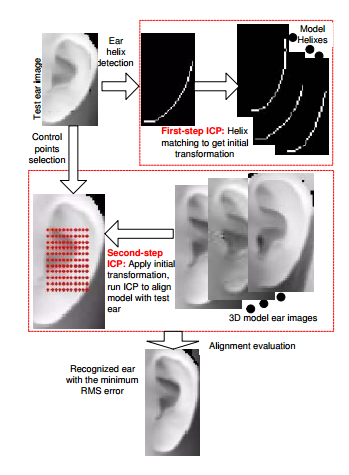
\includegraphics[scale=0.60]{res/icp_steps}
\caption{Алгоритм РСА}
\end{figure}

\end{frame}

\begin{frame}
\frametitle{Описание 3D распознавания уха}

Для каждой модели запускается IPC алгоритм для сравнения ее с тестовыми данными.
При этом облаком точек является облако точек спирали.
После этого мы имеем набор изометрий для каждой пары модель-тест. 
На втором шаге ICP алгоритма для лучшего распознавания сравнение производится по контрольным точкам для каждой пары модель-тест. 
Вычисляется среднее квадратичное (root mean square, RMS) зарегистрированных ошибок для каждой такой пары. 
Модель из пары с наименьшим RMS ошибок считается распознанным ухом

\end{frame}

%------------------------------------------------
\section{Совместное применение}
%------------------------------------------------

\begin{frame}
\frametitle{Эксперимент мульти-экземпляр}

\begin{itemize}
\item PCA алгоритм
\item Ранжировка расстояния косинусом Махаланобиса
\item Слияние результатов
\end{itemize}

\end{frame}

%------------------------------------------------

\begin{frame}
\frametitle{Таблица расстояний эксперимента}

Исследуется образец 02463. 

\begin{figure}[h!]
\centering
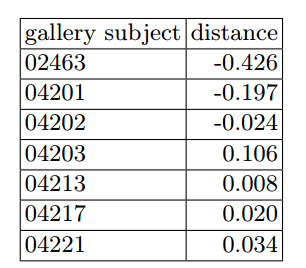
\includegraphics[scale=0.50]{res/distances_table}
\caption{Таблица дистанций}
\end{figure}

\end{frame}

%------------------------------------------------

\begin{frame}
\frametitle{Слияние результатов}

Можно выбрать разные способы слияния.
Например, суммировать расстояния, можно выставлять вес скажем 0.7 для уха и 0.3 для лица или наоборот. 
Так же можно выбирать минимальное значение.
В данном эксперименте результативность распознавания составила 100\%.
В свою очередь индивидуальное сопоставления при использовании PCA удавалось не во всех случаях.

\end{frame}

%------------------------------------------------

\begin{frame}
\frametitle{Пример сравнения индивидуального распознавания и со слиянием}

\begin{figure}[h!]
\centering
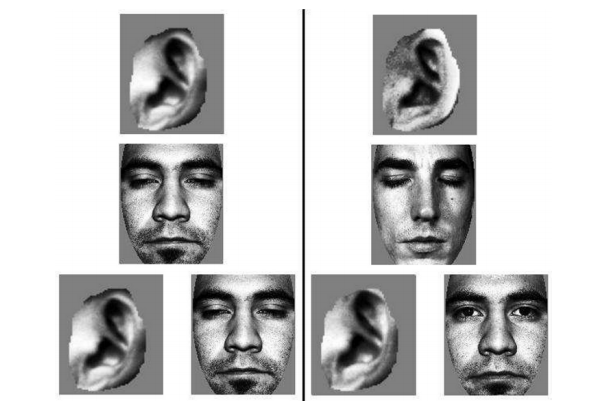
\includegraphics[scale=0.50]{res/ex_individual_failed}
\caption{Пример со слиянием и индивидуальное распознавание. Слева - образцы, справа найденные изображения из галереи}
\end{figure}

\end{frame}

%------------------------------------------------

\begin{frame}
\frametitle{Эксперимент мульти-модальный}

\begin{itemize}
\item мульти-экземпляр - ухо и лицо
\item мульти-сенсор - 2D и 3D
\item мульти-алгоритм - PCA и ICP
\end{itemize}

\end{frame}

%------------------------------------------------

\begin{frame}
\frametitle{Слияние результатов}

Для ICP результаты могут быть в диапазоне от 0 до бесконечности.
Для PCA от -1 до 1.
Для обоих случаев чем меньше, тем лучше.
Для нормализации результатов используется метод min-max.
Показатель вычисляются по формуле:
$s_i^\prime = \frac{s_i - min_i}{min_i - max_i}$
, где $min_i$ и $max_i$ - соответственно минимальные и максимальные значения из наборов.
Таким образом результирующий показатель будет в диапазоне от 0 до 1. 

\begin{figure}[h!]
\centering
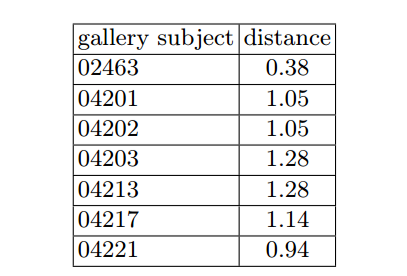
\includegraphics[scale=0.60]{res/distances_table_2}
\caption{Таблица дистанций}
\end{figure}

\end{frame}

%------------------------------------------------

\begin{frame}
\frametitle{Сравнение вариантов слияния}

Так же, как и в предыдущем примере возможны различные варианты слияния.

\begin{figure}[h!]
\centering
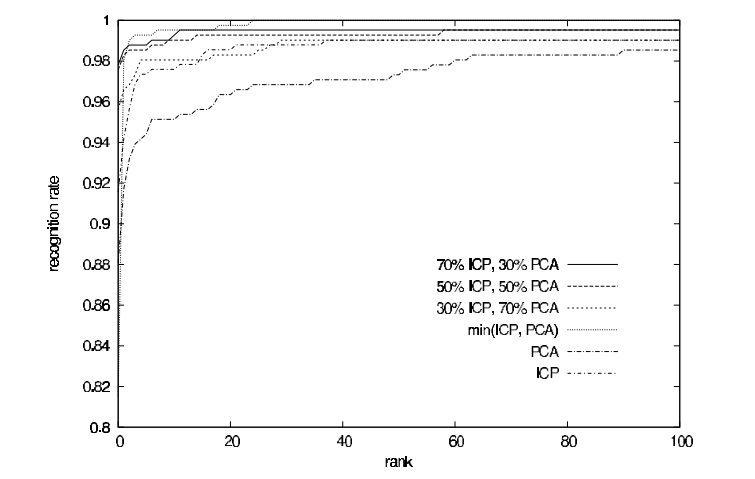
\includegraphics[scale=0.40]{res/fusion_rates}
\caption{Таблица дистанций}
\end{figure}

\end{frame}

\end{document} 
